\documentclass[12pt,a4paper]{article}
\usepackage[utf8]{inputenc}
\usepackage[T1]{fontenc}
\usepackage{amsmath,amsfonts,amssymb}%extensions de l'ams pour les mathématiques
\usepackage{graphicx}%pour insérer images et pdf entre autres
\usepackage[left=3.5cm,right=2cm,top=2cm,bottom=2.5cm]{geometry}%réglages des marges du document selon vos préférences ou celles de votre établissement
\usepackage[english]{babel}%pour un document en français
\usepackage{vmargin}
\usepackage{enumitem}
\usepackage[verbose]{wrapfig}
\usepackage{endnotes}
\usepackage{hyperref}
\usepackage{array}
\usepackage{multirow,makecell}
\setcellgapes{1pt}
\makegapedcells
\usepackage{lscape}

\begin{document}

\setcounter{tocdepth}{2}

\newenvironment{changemargin}[2]{\begin{list}{}{%
\setlength{\topsep}{0pt}%
\setlength{\leftmargin}{0pt}%
\setlength{\rightmargin}{0pt}%
\setlength{\listparindent}{\parindent}%
\setlength{\itemindent}{\parindent}%
\setlength{\parsep}{0pt plus 1pt}%
\addtolength{\leftmargin}{#1}%
\addtolength{\rightmargin}{#2}%
}\item }{\end{list}}

% définition de la taille de la feuille
\headsep 0cm
\textheight=23cm
\textwidth=16.8cm
\hoffset=0.0cm
\oddsidemargin 0cm
\evensidemargin 0cm
\voffset=0.5cm
\topmargin 0cm
\headheight 0.5cm

\begin{titlepage}
\begin{center}

\begin{figure}[h]
\vspace{-22mm}
\hspace{5mm}

\includegraphics[width=0.28\textwidth]{images/sorbonne.png}
\end{figure}
\begin{figure}[h]
\vspace{-35mm}
\hspace{110mm}

\includegraphics[width=0.22\textwidth]{images/spi.jpg}
\end{figure}
\vspace{-1mm}
\Huge{\textbf{\underline{\hspace{15cm}}}}\\

\large{\textit{Conception et optimisation des structures composites\\
Année universitaire 2018-2019\\
5AG12 \\ 
\vspace{-1cm}}}
\Huge{\textbf{\underline{\hspace{15cm}}}}\\

\vspace{40mm}


\Huge{\textbf{Optimisation d'une aile Delta en composite}}
%\begin{figure}[!ht]
%\begin{center}
%\hspace{5mm}
%\includegraphics[width=0.8\textwidth]{Composites.jpg}\centering
%\end{center}

%\vspace{5mm}
%\end{figure}
\underline{\hspace{15cm}}

\large{\vspace{70mm}\textit{Sorbonne Universités - Université Pierre et Marie Curie\\
Faculté des Sciences\\}
\large{\textit{Jean Schwager (3303438)}} \\}
\end{center}
\end{titlepage}

\newpage
\tableofcontents

%----------------------------------------------------------
%----------------------------------------------------------
%----------------------------------------------------------
%----------------------------------------------------------

\newpage

\section{Introduction}
oui materiaux composite c'est trop bien etc..
\section{Notre problème}
L'objectif de ce projet est de modéliser et d'optimiser la conception d'une aile delta en matériau composite stratifié. L'aile est composée d'une plaque en composite dont l'empilement des couches de stratifié peut être optimisée afin de maximiser la rigidité. 										  
\subsection{Géométrie du problème}
On considère une aile trapézoïdale d'envergure L et de cordes c0 et c1
Les calculs seront effectué pour les valeurs suivantes :
\begin{itemize}
\item $L=50$ cm
\item $c_0=0,5$ m
\item $c_1=0.5\times c_0$
\item $s=0.5$ m
\end{itemize} 
\begin{figure}[h]
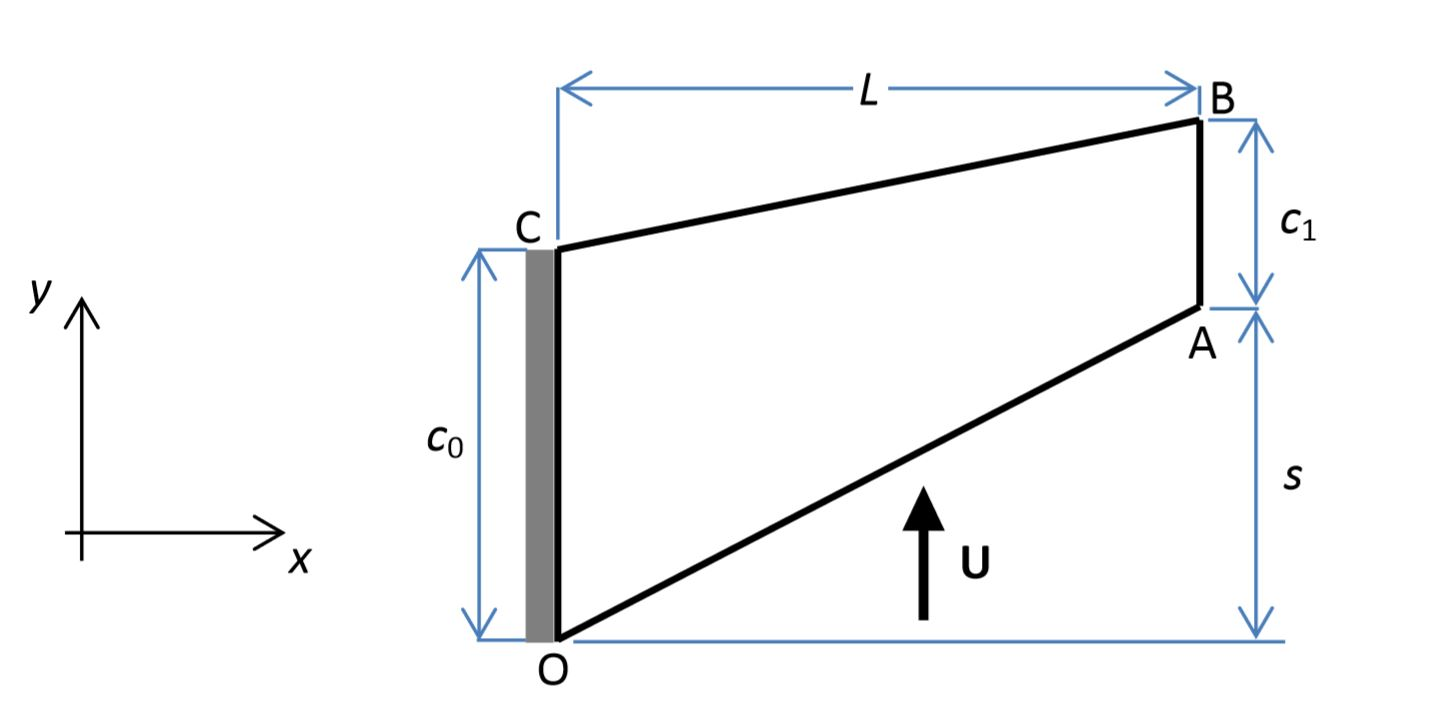
\includegraphics[scale=0.3]{images/geometrie.jpg} \centering
\caption{Géométrie du problème}
\end{figure}
\paragraph{}Pour la suite du calcul on considère que l'aile est encastré sur son bord gauche (segment CO)
\subsection{Matériau}
L'aile est fabriquée à partir d'un composite stratifié. Le matériau considéré est constitué de $N=16$ couches UD en carbone-époxyde T300/914. Chaque couche mesure $0,1$ mm d'épaisseur. la plaque aura donc une épaisseur $H = Nt$ avec $t$ l'épaisseur de chaque couche.
Les données du matériau sont les suivantes :
\begin{itemize}
\item $E_1=181$ GPa
\item $E_2=10.3$ GPa
\item $G_{12}=7.17$ GPa
\item $\nu_{12}=0.28$
\end{itemize}
\section{Résolution numérique du problème}
Afin de résoudre ce problème on va utiliser le logiciel de calcul par éléments finis Cast3m.
\subsection{Maillage}
L'aile est modélisé en 2 dimensions mais l'espace de sera bien en 3 dimensions. le maillage est constitué d'élément triangulaire à trois nœuds de type plaque mince de Kirschoff (DKT dans Cast3m). le nombre d'éléments du maillage doit être suffisant afin d'avoir un calcul convergé.
\subsection{Chargement}
\subsection{Matériau}
\section{Homogénéisation}
\section{Analyse et optimisation}
\section{Conclusion}
\end{document}
